\documentclass{standalone}
\usepackage{tikz}
\usetikzlibrary{patterns, positioning}

\begin{document}
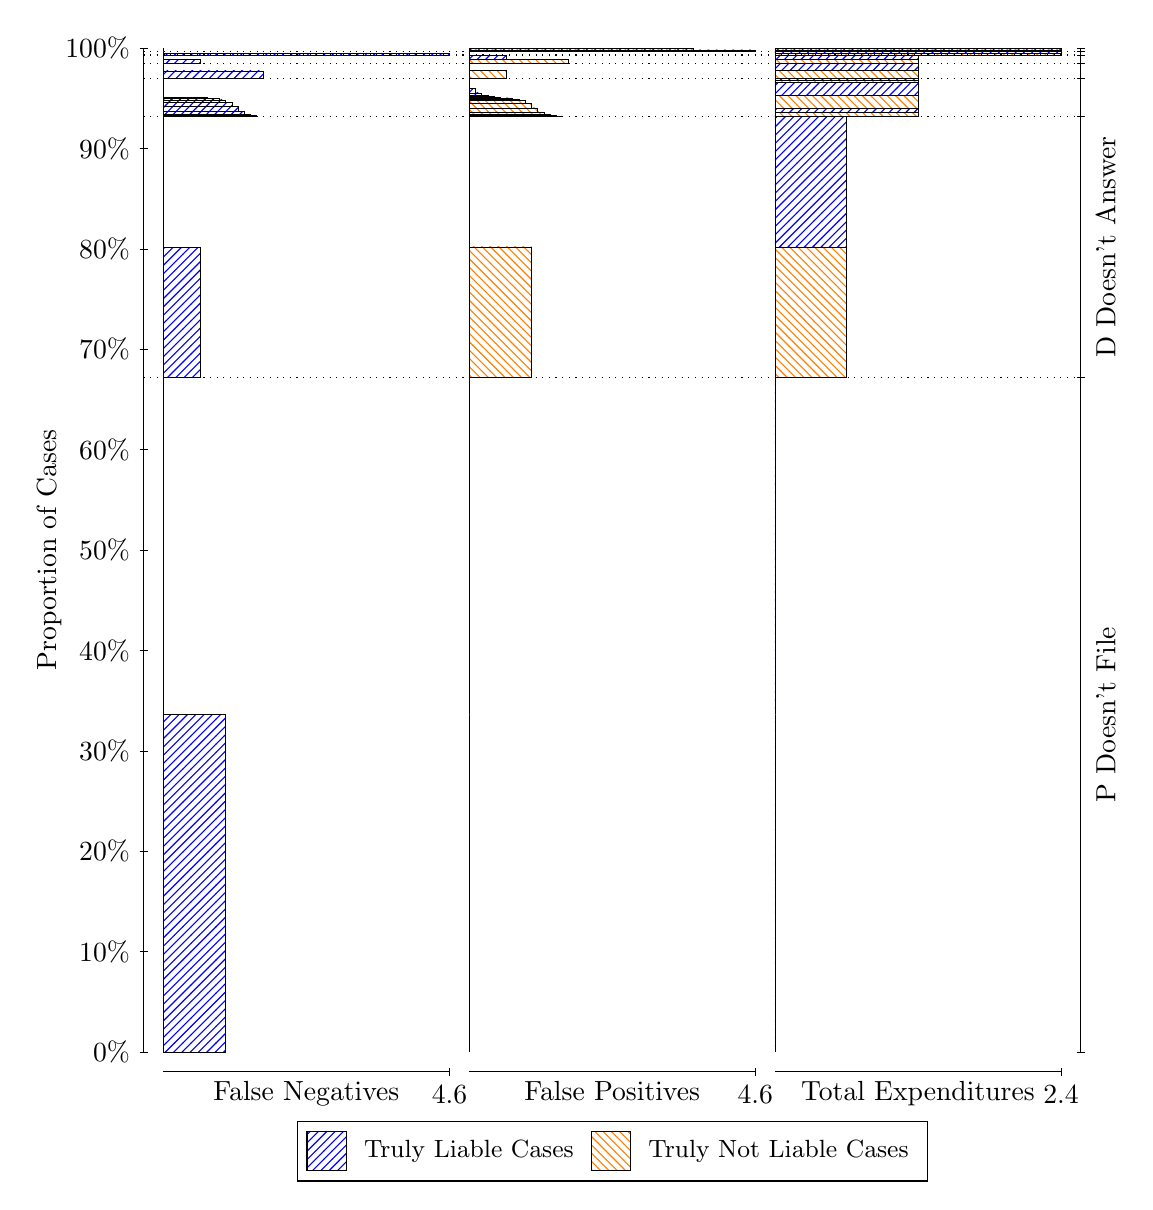
\begin{tikzpicture}
\draw[black, very thin] (1.5,1.75) -- (1.5,14.5);
\node[rotate=90, anchor=center] at (0.3, 8.125) {Proportion of Cases};
\draw[black, very thin] (1.45,1.75) -- (1.55,1.75);
\node[anchor=east] at (1.45, 1.75) {0\%};
\draw[black, very thin] (1.45,3.025) -- (1.55,3.025);
\node[anchor=east] at (1.45, 3.025) {10\%};
\draw[black, very thin] (1.45,4.3) -- (1.55,4.3);
\node[anchor=east] at (1.45, 4.3) {20\%};
\draw[black, very thin] (1.45,5.575) -- (1.55,5.575);
\node[anchor=east] at (1.45, 5.575) {30\%};
\draw[black, very thin] (1.45,6.85) -- (1.55,6.85);
\node[anchor=east] at (1.45, 6.85) {40\%};
\draw[black, very thin] (1.45,8.125) -- (1.55,8.125);
\node[anchor=east] at (1.45, 8.125) {50\%};
\draw[black, very thin] (1.45,9.4) -- (1.55,9.4);
\node[anchor=east] at (1.45, 9.4) {60\%};
\draw[black, very thin] (1.45,10.675) -- (1.55,10.675);
\node[anchor=east] at (1.45, 10.675) {70\%};
\draw[black, very thin] (1.45,11.95) -- (1.55,11.95);
\node[anchor=east] at (1.45, 11.95) {80\%};
\draw[black, very thin] (1.45,13.225) -- (1.55,13.225);
\node[anchor=east] at (1.45, 13.225) {90\%};
\draw[black, very thin] (1.45,14.5) -- (1.55,14.5);
\node[anchor=east] at (1.45, 14.5) {100\%};

\draw[black, very thin] (13.4,1.75) -- (13.4,14.5);
\draw[black, very thin] (13.35,1.75) -- (13.45,1.75);
\node[anchor=west] at (13.35, 1.75) {};
\draw[black, very thin] (13.35,10.317) -- (13.45,10.317);
\node[anchor=west] at (13.35, 10.317) {};
\draw[black, very thin] (13.35,13.627) -- (13.45,13.627);
\node[anchor=west] at (13.35, 13.627) {};
\draw[black, very thin] (13.35,14.116) -- (13.45,14.116);
\node[anchor=west] at (13.35, 14.116) {};
\draw[black, very thin] (13.35,14.306) -- (13.45,14.306);
\node[anchor=west] at (13.35, 14.306) {};
\draw[black, very thin] (13.35,14.411) -- (13.45,14.411);
\node[anchor=west] at (13.35, 14.411) {};
\draw[black, very thin] (13.35,14.456) -- (13.45,14.456);
\node[anchor=west] at (13.35, 14.456) {};
\draw[black, very thin] (13.35,14.5) -- (13.45,14.5);
\node[anchor=west] at (13.35, 14.5) {};

\draw[black, very thin, pattern color=blue, pattern=north east lines] (1.75,1.75) rectangle (2.5399,6.0335);
\draw[black, very thin, pattern color=orange, pattern=north west lines] (1.75,6.0335) rectangle (1.75,10.317);
\draw[black, very thin, pattern color=blue, pattern=north east lines] (1.75,10.317) rectangle (2.2239,11.97);
\draw[black, very thin, pattern color=orange, pattern=north west lines] (1.75,11.97) rectangle (1.75,13.627);
\draw[black, very thin, pattern color=blue, pattern=north east lines] (1.75,13.627) rectangle (2.9348,13.644);
\draw[black, very thin, pattern color=blue, pattern=north east lines] (1.75,13.644) rectangle (2.8558,13.654);
\draw[black, very thin, pattern color=blue, pattern=north east lines] (1.75,13.654) rectangle (2.7768,13.7);
\draw[black, very thin, pattern color=blue, pattern=north east lines] (1.75,13.7) rectangle (2.6978,13.758);
\draw[black, very thin, pattern color=blue, pattern=north east lines] (1.75,13.758) rectangle (2.6188,13.812);
\draw[black, very thin, pattern color=blue, pattern=north east lines] (1.75,13.812) rectangle (2.5399,13.841);
\draw[black, very thin, pattern color=blue, pattern=north east lines] (1.75,13.841) rectangle (2.4609,13.859);
\draw[black, very thin, pattern color=blue, pattern=north east lines] (1.75,13.859) rectangle (2.3819,13.867);
\draw[black, very thin, pattern color=blue, pattern=north east lines] (1.75,13.867) rectangle (2.3029,13.874);
\draw[black, very thin, pattern color=orange, pattern=north west lines] (1.75,13.874) rectangle (1.75,14.116);
\draw[black, very thin, pattern color=blue, pattern=north east lines] (1.75,14.116) rectangle (3.0138,14.21);
\draw[black, very thin, pattern color=orange, pattern=north west lines] (1.75,14.21) rectangle (1.75,14.306);
\draw[black, very thin, pattern color=blue, pattern=north east lines] (1.75,14.306) rectangle (2.2239,14.36);
\draw[black, very thin, pattern color=orange, pattern=north west lines] (1.75,14.36) rectangle (1.75,14.411);
\draw[black, very thin, pattern color=blue, pattern=north east lines] (1.75,14.411) rectangle (5.3833,14.431);
\draw[black, very thin, pattern color=orange, pattern=north west lines] (1.75,14.431) rectangle (1.75,14.456);
\draw[black, very thin, pattern color=orange, pattern=north west lines] (1.75,14.456) rectangle (1.75,14.476);
\draw[black, very thin, pattern color=blue, pattern=north east lines] (1.75,14.476) rectangle (1.75,14.5);
\draw[black, very thin, pattern color=orange, pattern=north west lines] (5.6333,1.75) rectangle (5.6333,6.0335);
\draw[black, very thin, pattern color=blue, pattern=north east lines] (5.6333,6.0335) rectangle (5.6333,10.317);
\draw[black, very thin, pattern color=orange, pattern=north west lines] (5.6333,10.317) rectangle (6.4232,11.974);
\draw[black, very thin, pattern color=blue, pattern=north east lines] (5.6333,11.974) rectangle (5.6333,13.627);
\draw[black, very thin, pattern color=orange, pattern=north west lines] (5.6333,13.627) rectangle (6.8181,13.634);
\draw[black, very thin, pattern color=orange, pattern=north west lines] (5.6333,13.634) rectangle (6.7391,13.641);
\draw[black, very thin, pattern color=orange, pattern=north west lines] (5.6333,13.641) rectangle (6.6601,13.659);
\draw[black, very thin, pattern color=orange, pattern=north west lines] (5.6333,13.659) rectangle (6.5812,13.688);
\draw[black, very thin, pattern color=orange, pattern=north west lines] (5.6333,13.688) rectangle (6.5022,13.74);
\draw[black, very thin, pattern color=orange, pattern=north west lines] (5.6333,13.74) rectangle (6.4232,13.796);
\draw[black, very thin, pattern color=orange, pattern=north west lines] (5.6333,13.796) rectangle (6.3442,13.84);
\draw[black, very thin, pattern color=orange, pattern=north west lines] (5.6333,13.84) rectangle (6.2652,13.85);
\draw[black, very thin, pattern color=orange, pattern=north west lines] (5.6333,13.85) rectangle (6.1862,13.868);
\draw[black, very thin, pattern color=blue, pattern=north east lines] (5.6333,13.868) rectangle (6.0283,13.876);
\draw[black, very thin, pattern color=blue, pattern=north east lines] (5.6333,13.876) rectangle (5.9493,13.883);
\draw[black, very thin, pattern color=blue, pattern=north east lines] (5.6333,13.883) rectangle (5.8703,13.901);
\draw[black, very thin, pattern color=blue, pattern=north east lines] (5.6333,13.901) rectangle (5.7913,13.93);
\draw[black, very thin, pattern color=blue, pattern=north east lines] (5.6333,13.93) rectangle (5.7123,13.985);
\draw[black, very thin, pattern color=blue, pattern=north east lines] (5.6333,13.985) rectangle (5.6333,14.116);
\draw[black, very thin, pattern color=orange, pattern=north west lines] (5.6333,14.116) rectangle (6.1072,14.213);
\draw[black, very thin, pattern color=blue, pattern=north east lines] (5.6333,14.213) rectangle (5.6333,14.306);
\draw[black, very thin, pattern color=orange, pattern=north west lines] (5.6333,14.306) rectangle (6.8971,14.358);
\draw[black, very thin, pattern color=blue, pattern=north east lines] (5.6333,14.358) rectangle (6.1072,14.411);
\draw[black, very thin, pattern color=orange, pattern=north west lines] (5.6333,14.411) rectangle (5.6333,14.436);
\draw[black, very thin, pattern color=blue, pattern=north east lines] (5.6333,14.436) rectangle (5.6333,14.456);
\draw[black, very thin, pattern color=orange, pattern=north west lines] (5.6333,14.456) rectangle (9.2667,14.476);
\draw[black, very thin, pattern color=blue, pattern=north east lines] (5.6333,14.476) rectangle (8.4768,14.5);
\draw[black, very thin, pattern color=orange, pattern=north west lines] (9.5167,1.75) rectangle (9.5167,6.0335);
\draw[black, very thin, pattern color=blue, pattern=north east lines] (9.5167,6.0335) rectangle (9.5167,10.317);
\draw[black, very thin, pattern color=orange, pattern=north west lines] (9.5167,10.317) rectangle (10.425,11.974);
\draw[black, very thin, pattern color=blue, pattern=north east lines] (9.5167,11.974) rectangle (10.425,13.627);
\draw[black, very thin, pattern color=orange, pattern=north west lines] (9.5167,13.627) rectangle (11.333,13.679);
\draw[black, very thin, pattern color=blue, pattern=north east lines] (9.5167,13.679) rectangle (11.333,13.733);
\draw[black, very thin, pattern color=orange, pattern=north west lines] (9.5167,13.733) rectangle (11.333,13.898);
\draw[black, very thin, pattern color=blue, pattern=north east lines] (9.5167,13.898) rectangle (11.333,14.065);
\draw[black, very thin, pattern color=orange, pattern=north west lines] (9.5167,14.065) rectangle (11.333,14.091);
\draw[black, very thin, pattern color=blue, pattern=north east lines] (9.5167,14.091) rectangle (11.333,14.116);
\draw[black, very thin, pattern color=orange, pattern=north west lines] (9.5167,14.116) rectangle (11.333,14.213);
\draw[black, very thin, pattern color=blue, pattern=north east lines] (9.5167,14.213) rectangle (11.333,14.306);
\draw[black, very thin, pattern color=orange, pattern=north west lines] (9.5167,14.306) rectangle (11.333,14.358);
\draw[black, very thin, pattern color=blue, pattern=north east lines] (9.5167,14.358) rectangle (11.333,14.411);
\draw[black, very thin, pattern color=orange, pattern=north west lines] (9.5167,14.411) rectangle (13.15,14.436);
\draw[black, very thin, pattern color=blue, pattern=north east lines] (9.5167,14.436) rectangle (13.15,14.456);
\draw[black, very thin, pattern color=orange, pattern=north west lines] (9.5167,14.456) rectangle (13.15,14.476);
\draw[black, very thin, pattern color=blue, pattern=north east lines] (9.5167,14.476) rectangle (13.15,14.5);
\draw[black, dotted] (1.5,10.317) -- (13.4,10.317);
\draw[black, dotted] (1.5,13.627) -- (13.4,13.627);
\draw[black, dotted] (1.5,14.116) -- (13.4,14.116);
\draw[black, dotted] (1.5,14.306) -- (13.4,14.306);
\draw[black, dotted] (1.5,14.411) -- (13.4,14.411);
\draw[black, dotted] (1.5,14.456) -- (13.4,14.456);
\draw[black, very thin] (1.75,1.5) -- (5.3833,1.5);
\node[anchor=north] at (3.5667, 1.5) {False Negatives};
\draw[black, very thin] (5.3833,1.45) -- (5.3833,1.55);
\node[anchor=north] at (5.3833, 1.45) {4.6};

\draw[black, very thin] (5.6333,1.5) -- (9.2667,1.5);
\node[anchor=north] at (7.45, 1.5) {False Positives};
\draw[black, very thin] (9.2667,1.45) -- (9.2667,1.55);
\node[anchor=north] at (9.2667, 1.45) {4.6};

\draw[black, very thin] (9.5167,1.5) -- (13.15,1.5);
\node[anchor=north] at (11.333, 1.5) {Total Expenditures};
\draw[black, very thin] (13.15,1.45) -- (13.15,1.55);
\node[anchor=north] at (13.15, 1.45) {2.4};

\node[black, centered, rotate=90] at (13.72, 6.0335) {P Doesn't File};
\node[black, centered, rotate=90] at (13.72, 11.972) {D Doesn't Answer};






\draw (7.449999999999999,1.5) node[draw=none] (baseCoordinate) {};
\begin{scope}[align=center]
        \matrix[scale=0.5, draw=black, below=0.5cm of baseCoordinate, nodes={draw}, column sep=0.1cm]{
            \node[rectangle, draw, minimum width=0.5cm, minimum height=0.5cm, pattern=north east lines, pattern color=blue] {}; &
            \node[draw=none, font=\small] (B) {Truly Liable Cases}; &
            \node[rectangle, draw, minimum width=0.5cm, minimum height=0.5cm, pattern=north west lines, pattern color=orange] {}; &
            \node[draw=none, font=\small] (B) {Truly Not Liable Cases}; \\
            };
\end{scope}

\end{tikzpicture}
\end{document}